\documentclass[letter]{article}

%% Language and font encodings
\usepackage[english]{babel}
\usepackage[utf8x]{inputenc}
\usepackage[T1]{fontenc}
\usepackage{listings}
\usepackage{stmaryrd}
\usepackage{pgfplots}

%% Sets page size and margins
\usepackage[top=2cm,bottom=2cm,left=3cm,right=3cm,marginparwidth=1.75cm]{geometry}

%% Useful packages
\usepackage{amsmath}
\usepackage{amsfonts}
\usepackage{amssymb}
\usepackage{amsthm}
\usepackage{graphicx}
\usepackage[colorinlistoftodos]{todonotes}
%\usepackage[colorlinks=true, allcolors=blue]{hyperref}
\usepackage{array}
\usepackage[shortlabels]{enumitem}
\usepackage[final]{pdfpages}
\usepackage[normalem]{ulem}
\usepackage{cancel}
\usepackage{xspace,mdwlist}
\usepackage{algorithmic}
\usepackage{mathtools}
\usetikzlibrary{calc}

\usepackage{courier} %% Sets font for listing as Courier.
\usepackage{listings, xcolor}
\lstset{
tabsize = 4, %% set tab space width
showstringspaces = false, %% prevent space marking in strings, string is defined as the text that is generally printed directly to the console
numbers = left, %% display line numbers on the left
commentstyle = \color{green}, %% set comment color
keywordstyle = \color{blue}, %% set keyword color
stringstyle = \color{red}, %% set string color
rulecolor = \color{black}, %% set frame color to avoid being affected by text color
basicstyle = \small \ttfamily , %% set listing font and size
breaklines = true, %% enable line breaking
numberstyle = \tiny,
}



\DeclarePairedDelimiter{\ceil}{\lceil}{\rceil}
\DeclarePairedDelimiter{\floor}{\lfloor}{\rfloor}

\newtheorem{theorem}{Theorem}[section]
\newtheorem*{claim}{Claim}
\DeclareMathOperator*{\argmin}{\arg\!\min}

\def\coursename{CS 201: Data Structures}

%% make title box
\newcommand{\header}[1]{%
	\begin{center}
		\fbox{
			\begin{minipage}{6in}
				\textbf{\coursename} \hfill       \\
				\textit{#1} \hfill \textit{\today}
			\end{minipage}
		}
	\end{center}
	\vspace*{4mm}
}

\def\problem#1#2#3{
\fbox{
\begin{minipage}{0.8\textwidth}
{\sc #1:}

\begin{description*}
\item[Given:] #2
\item[Find:] #3
\end{description*}
\end{minipage}
}
\bigskip
}


\begin{document}

\header{Week 4: big-O, stacks, queues}

\begin{enumerate}[1.] 
    \item Big-O foundation
    \begin{itemize}
        \item [(a)] When evaluating the efficiency of a program, why do we use big-O notation instead of the \textit{performance}, which is the actual time to run the program?\\\\
            Performance depends on what machine we are running the program on, and how many tasks the current machine is running. Thus, performance is an unreliable way to measure program efficiency. Big-O is better because it is constant across different machine type or the number of running tasks.
        \item [(b)] In one sentence, what does big-O measure?\\\\
            How execution time, or the number of operations, increases with input size.
        \item [(c)] Provide the big-O notation and the names (constant, linear, quadratic, or logarithmic) for each function:\\\\

        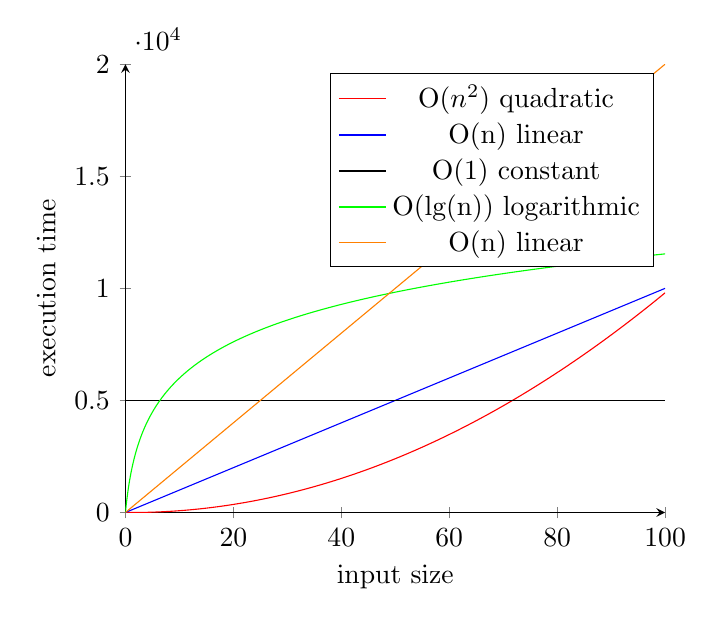
\begin{tikzpicture}
\begin{axis}[
    axis lines = left,
    xlabel = input size,
    ylabel = execution time,
]
%Below the red parabola is defined
\addplot [
    domain=0:100, 
    samples=500, 
    color=red,
]
{x^2 - 2*x};
\addlegendentry{O($n^2$) quadratic}
\addplot [
    domain=0:100, 
    samples=500, 
    color=blue,
    ]
    {100*x};
    \addlegendentry{O(n) linear}
\addplot [
    domain=0:100, 
    samples=500, 
    color=black,
    ]
    {5000};
    \addlegendentry{O(1) constant}
\addplot [
    domain=0:100, 
    samples=500, 
    color=green,
    ]
    {ln(x+1)* 2500};
    \addlegendentry{O(lg(n)) logarithmic}
\addplot [
    domain=0:100, 
    samples=500, 
    color=orange,
    ]
    {200*x};
    \addlegendentry{O(n) linear}
\end{axis}
\end{tikzpicture}

    \item [(d)] Arrange the functions in (c) in terms of how fast it grows as the input size increases to infinity.

    Slowest growth -> O(1) -> O(lg(n)) -> O(n) -> O($n^2$) -> fastest growth

    \end{itemize}

    \newpage
    \item Big-O Practice
    \begin{itemize}
    \item [(a)] What is the runtime complexity of the following LinkedList method? O(n)

    \begin{lstlisting}[language = Java , frame = trBL , firstnumber = 0 , escapeinside={(*@}{@*)}]
public int potato(int numItems) {
    int someNum = 0;
    Node<E> temp = head;
    while (temp != null) {
        if ((temp.data).equals(item)) { //You can assume that equals() is O(1)
            break;
        }
        temp = temp.next;
        someNum++;
    }
    if (count >= numItems) {
        return -1;
    }
    return someNum;
}
    \end{lstlisting}

    \item [(b)] What is the runtime complexity of the following LinkedList method? O(1)

    \begin{lstlisting}[language = Java , frame = trBL , firstnumber = 0 , escapeinside={(*@}{@*)}]
public boolean strawberry(Node<E> node) {
    if (node.next != null) {
        return true;
    }
    return false;
}
    \end{lstlisting}

    \item [(c)] What is the runtime complexity of the following method? (This one is challenging, so feel free to ask for hints!) O($n^2$)

    \begin{lstlisting}[language = Java , frame = trBL , firstnumber = 0 , escapeinside={(*@}{@*)}]
public Integer[] whatIsThis(int numItems) {
    Integer[] numArray = new Integer[numItems];
    for (int i=0; i < numItems; i++) {
        int sum = 0;
        for (int j = i; j < numItems; j++) {
            sum += j;
        }
        numArray[i] = sum;
    }
    return numArray;
}
    \end{lstlisting}
    \end{itemize}
\newpage
    \item Stacks and Queues foundation
    \begin{itemize}
        \item [(a)] True/False: Stack is a LIFO (last in first out) ADT, while queue is a FIFO (first in first out) ADT. (TRUE)
        \item [(b)] (Adapted from Koffman-Wolfgang) What is the output of the following:

    \begin{lstlisting}[language = Java , frame = trBL , firstnumber = 0 , escapeinside={(*@}{@*)}]
Stack<String> myStack = new Stack<string>();
myStack.push("meow");
myStack.push("woof");
myStack.push("moo");
myStack.push("oink");
String sound = myStack.peek();

while (!myStack.isEmpty()) { //isEmpty returns true if stack is empty
    System.out.println(names.pop());
}
System.out.println(sound);
    \end{lstlisting}
    oink\\
    moo\\
    woof\\
    meow\\
    oink
    \item [(c)] (Adapted from Koffman-Wolfgang) What is the output of the following:

    \begin{lstlisting}[language = Java , frame = trBL , firstnumber = 0 , escapeinside={(*@}{@*)}]
Queue<String> myQueue = new Queue<string>();
myQueue.enqueue("meow");
myQueue.enqueue("woof");
myQueue.enqueue("moo");
myQueue.enqueue("oink");
String sound = myStack.peek();

while (!myStack.isEmpty()) { //isEmpty returns true if stack is empty
    System.out.println(names.dequeue());
}
System.out.println(sound);
    \end{lstlisting}
    meow\\
    woof\\
    moo\\
    oink\\
    meow
    \end{itemize}
    
    \item Dynamic array vs linked lists
    \begin{itemize}
        \item [(a)] What are the advantages and disadvantages of using a dynamic array vs linked list for a stack implementation?\\

        Dynamic array advantage: wastes less memory because, unlike linked lists, there's no need to store the pointer to the next node.\\
        Dynamic array disadvantage: need to resize array, so push(item) won't be O(1) every time.\\

        Linked list advantage: push, pop, and peek are all O(1)\\
        Linked list disadvantage: the extra pointer to next node costs extra memory
        
        \item [(b)] What are the advantages and disadvantages of using a dynamic array vs linked list for a queue implementation?\\

        Same as above.
        
    \end{itemize}

    \newpage
    \item (Adapted from Koffman-Wolfgang) A palindrome is a string which reads the same in either direction: left to right or right to left. For example, "kayak", "racecar" are palindromes. Write a method \textbf{public static boolean isPalindrome(String word)} that returns true if \textbf{word} is a palindrome, and false otherwise. You must use a stack in this method. 

    \begin{lstlisting}[language = Java , frame = trBL , firstnumber = 0 , escapeinside={(*@}{@*)}]
public static boolean isPalindrome(String word) {
    Stack<Character> myStack = new Stack<Character>();
    
    //To figure out whether word is a palindrome, we only need to compare whether the first half is the second half in reverse, or vice versa. 
    
    int len = word.length();
    
    //Loop over the first half
    for (int i = 0; i < (len / 2); i++) { 
        myStack.push(word.charAt(i));
    }
    //Loop over each character in the second half of the word, see if it matches the first half in reverse.
    for (int i = (len/2) + len%2; i < len; i++) {
        Character current = myStack.pop();
        if (!current.equals(word.charAt(i))) {
            return false; 
        }
    }
    return true;
}
    \end{lstlisting}

    
    \item Suppose we have a queue myQueue ["c","a","b"] where front is at index 1, rear at index 0. 
    \begin{itemize}
        \item [(a)] Suppose I perform enqueue("d") on myQueue. Draw newArray and indicate the value of i for each iteration of the for loop. \\\\

        1st iteration: i = 1
        dataArray = ["c", "a", "b"]
        newArray = [  ,"a",  ,  ,  ,  ]

        2nd iteration: i = 2
        dataArray = ["c", "a", "b"]
        newArray = [  ,"a","b",  ,  ,  ]

        3rd iteration: i = 3
        dataArray = ["c", "a", "b"]
        newArray = [  ,"a","b","c",  ,  ]
        
        \item [(b)] After each method execution, what is the value of rear for myQueue?
            \begin{itemize}
                \item myQueue.enqueue("d"); rear = 4
                \item myQueue.enqueue("e"); rear = 5
                \item myQueue.enqueue("f"); rear = 0
            \end{itemize}
        
    \end{itemize} 

    \begin{lstlisting}[language = Java , frame = trBL , firstnumber = 0 , escapeinside={(*@}{@*)}]
public class Queue {
    int numItems;
    int capacity; //the total number of slots in our E[] array
    E[] dataArray;
    int front; //Index of the oldest item in the queue
    int rear; //Index of the most recent item in the queue
    public void enqueue(E item) {
        //expand the array if it is full
        if (numItems == capacity) {
            newArray = (E[]) new Object[capacity*2];
            for (int i = front; i < front + numItems; i++) {
                newArray[i] = data[i%capacity];
            }
            dataArray = newArray;
            rear = front + numItems; //adjust rear to its correct number
            capacity *= 2; //update the array capacity
        }
        //If we don't have to expand the array, then rear is gonna be a bit different
        else {
            rear = (rear + 1) % capacity;
        }
        data[rearIndex] = item; //finally, add the new item at index rear
    }
}

    \end{lstlisting}
\end{enumerate}
\end{document}
